\documentclass[varwidth=true, border=10pt]{standalone}
\usepackage{tkz-euclide}
\newcommand{\iu}{{i\mkern1mu}} % imaginary unit

\begin{document}
\usetkzobj{all}
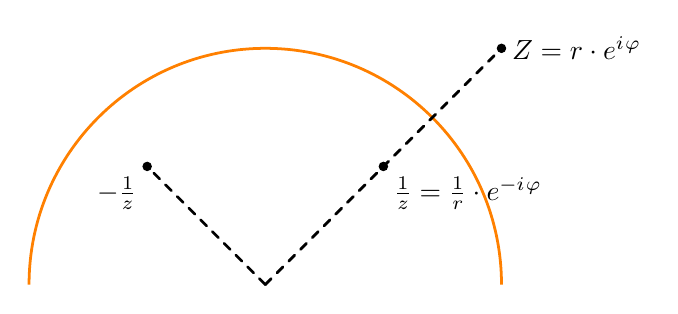
\begin{tikzpicture}[scale=3]
    \tkzSetUpPoint[shape=circle,size=3,color=black,fill=black]
    \tkzSetUpLine[line width=1]
    \tkzInit[xmax=1.2,ymax=1,xmin=-1.2,ymin=0]
    \tkzDefPoints{1/1/Z,0.5/0.5/dZ,-0.5/0.5/ndZ,0/0/O}
    \tkzDrawArc[R,line width=1pt,color=orange](O,1 cm)(0,180)
    \tkzAxeXY

    \tkzDrawPoints(Z, dZ, ndZ)
    \tkzLabelPoint[right](Z){$Z = r \cdot e^{\iu \varphi}$}
    \tkzLabelPoint[below right](dZ){$\frac{1}{z} = \frac{1}{r} \cdot e^{-\iu \varphi}$}
    \tkzLabelPoint[below left](ndZ){$-\frac{1}{z}$}
    \tkzDrawSegments[dashed](O,Z)
    \tkzDrawSegments[dashed](O,ndZ)
\end{tikzpicture}
\end{document}
